\chapter{学位论文书写注意事项及错误检查}\label{appendix:checkingthesis}
\parwords{写在前面(资料收集于互联网和部分书籍,仅供参考)}

同学们撰写学位论文时,常常犯一些错误,有些是格式错误,有些是内容错误。本文列举 30 种常见的错误,辅之以实例及修正方法。
本文的正确使用方法是:按照 30 个检查点,逐项对照检查;有则改之,无则加勉。

参考资料:《科技书刊标准化18讲》

\section{中文摘要}

摘要内容要求在800~1200字。
摘要是以提供文献内容梗概为目的,不加评论和补充解释,简明、确切地记述文献重要内容的短文。其要素一般包括:
 (1)目的——研究、研制、调查等的前提、目的和任务,所涉及的主要范围;
 (2)方法——所用的原理、理论、条件、对象、材料、工艺、结构、手段、装备、程序等;
 (3)结果——实验的、研究的结果,数据,被确定的关系,观察结果,得到的效果,性能等;
 (4)结论——结果的分析、研究、比较、评价、应用,提出的问题,今后的课题,假设,启发,建议,预测等; 

写摘要时不得简单地重复题名中已有的信息,要排除在本学科领域中已成常识的内容,要用第三人称的写法。
应采用“对……进行了研究”、“报告了……现状”、“进行了……调查”等记述方法,不使用“本文”、“作者”等作为主语。
摘要的第一句不要与题目重复;取消或减少背景信息,只表示新情况、新内容;不说空洞的词句,
如“本文所讨论的工作是对过去×××的一个极大地改进”、“本工作首次实现了……”、“经检索尚未发现与本文类似的工作”等;
此外,作者的打算及未来的计划不能纳入摘要。

在摘要的最下方另起一行,列出3~5个关键词,以关键字与课题间关联性由强到弱顺序排列,关键词之间用逗号相隔,结束处不用标点符号。

\begin{itemize}
\item \emph{陈述贡献时,“我们”应改成“本项研究”或者“本文”。}
\begin{figure}[!htpb]
\centering
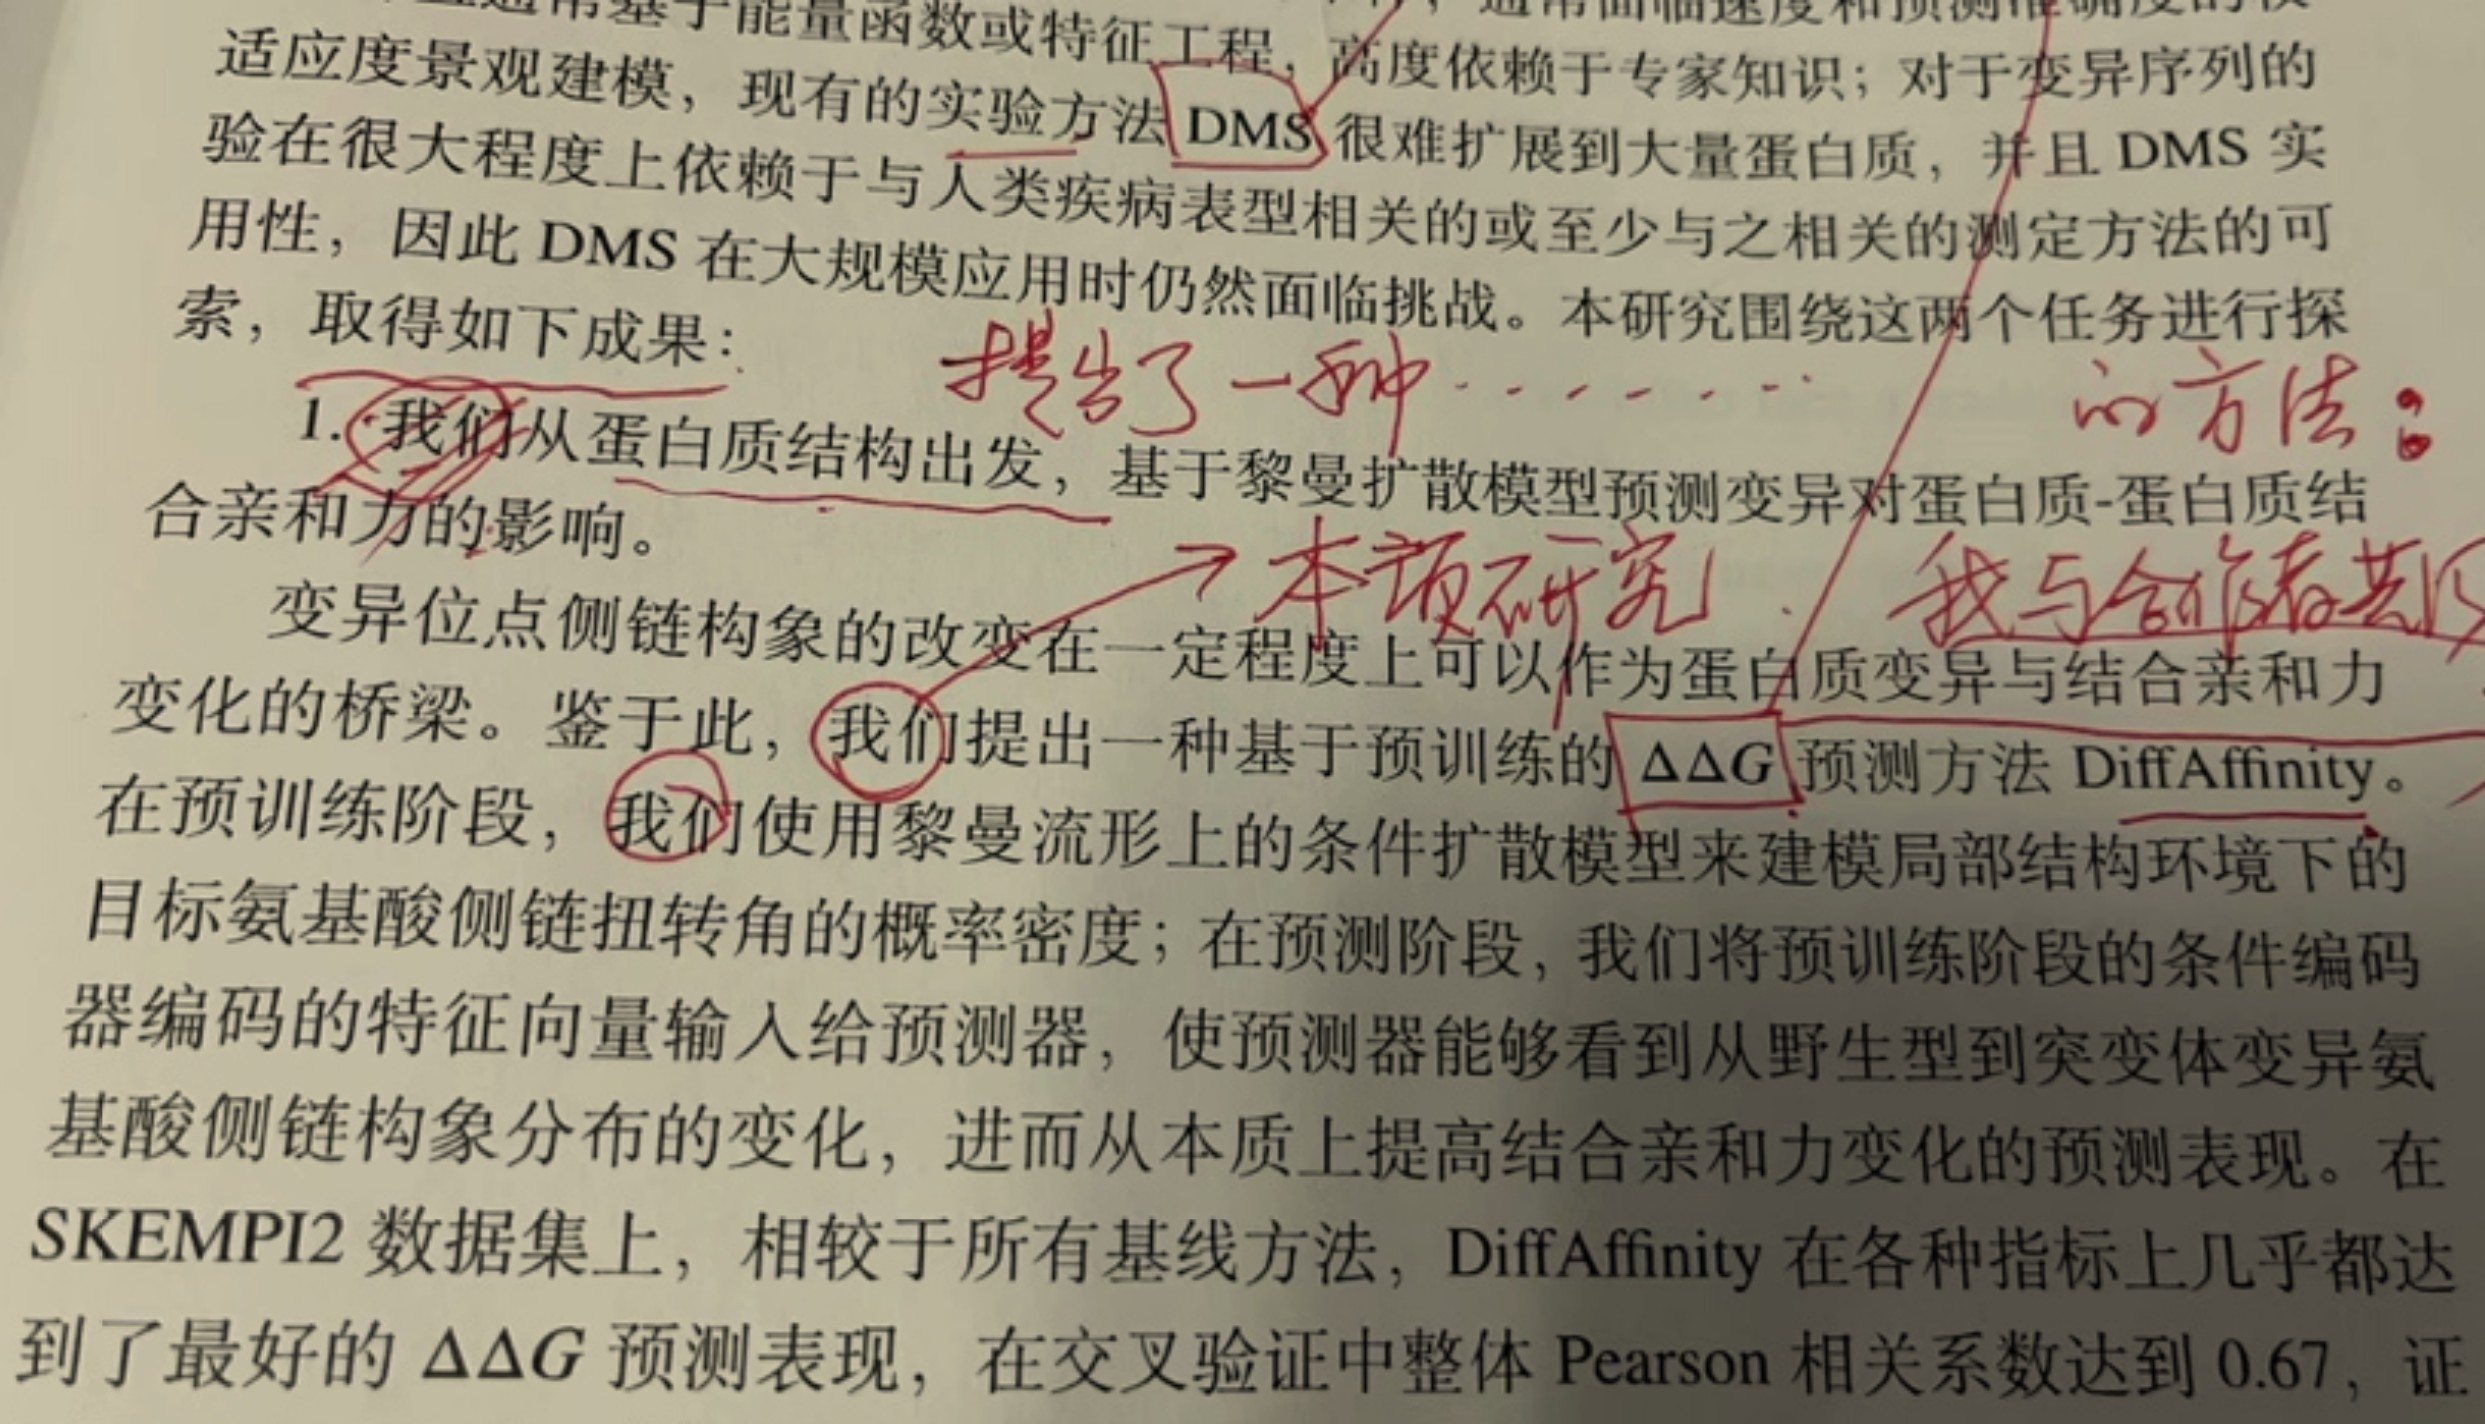
\includegraphics[scale=0.3]{doc/figures/chk01.jpg}
\caption{中文摘要错误之“我们”}
\label{fig:abstract-error-we}
\end{figure}

与期刊/会议论文(paper)不同,学位论文(thesis)是个人作品,供学位评定之用,因此具有浓厚的个人色彩。
为厘清其他个人或集体的贡献,学位论文中的前面都会包含一个声明,比如“学位论文系本人在导师指导下独立进行研究工作取得的成果;对本论文所涉及的研究工
作做出贡献的其他个人或集体,均已在文中以明确方式标明或致谢。”因此,在学位论文中陈述贡献时,不能用“我们”。关于这一点,剑桥大学专门写了一句话:
"For a dissertation with one author, do not use the "editorial we" in place of "I".The use of "we" by a single author is outrageously pretentious.".

解决方法:以“本文”或“本项研究”代替“我们”;在英文中,使用“Our research shows....”或“The conclusions made from this analysis are ....”替代“we”。

需要注意的是,这不是说通篇不能使用“我们”---“我们”有两层含义,一是表示“作者及其合作者”,即:“With the assistance of my colleagues, I designed …”,二是表示“作者和读者”,即:“the readers”。在采用第二个义项时,可以使用“我们”。


\item \emph{描述已完成工作时,建议采用如例\ref{examp:contribution-item}给出的“冒号式、分点陈述”格式,使用“提出了一种/开发了一套/构建了一个”等说法。}
\begin{figure}[!htpb]
\centering
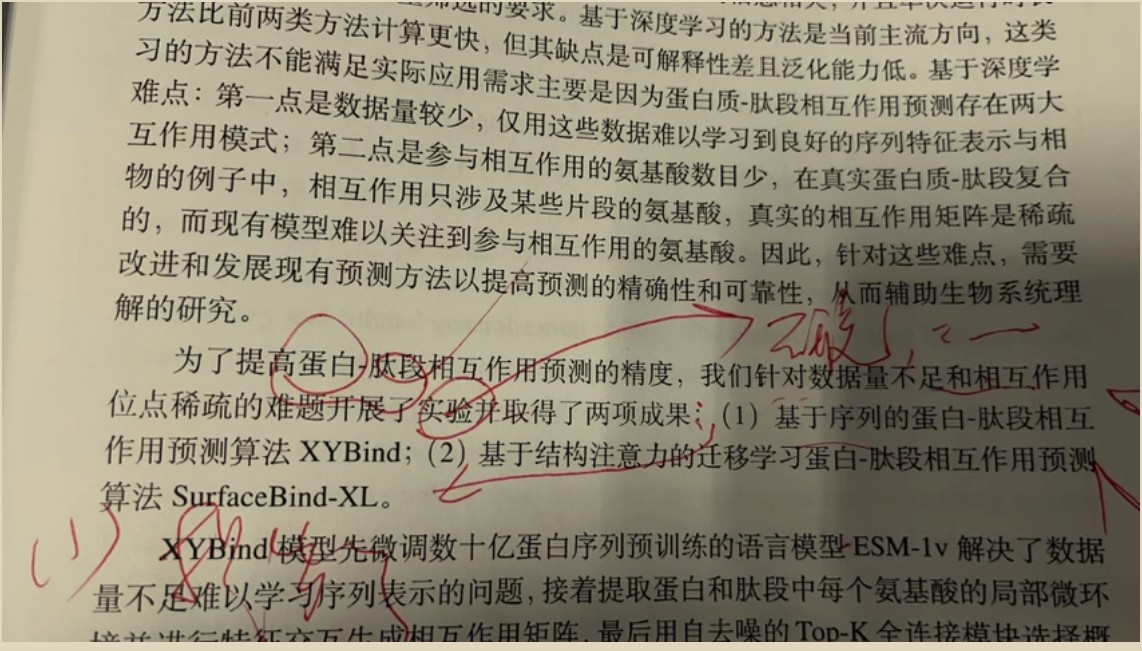
\includegraphics[scale=0.65]{doc/figures/chk02.jpg}
\caption{中文摘要错误之贡献分条列出}
\label{fig:abstract-error-contribution}
\end{figure}
\begin{example}\label{examp:contribution-item}
本项研究取得了如下成果:
\begin{enumerate}
    \item 提出了一种 xxxx 算法:详细陈述目标、基本思想、性能等。
    \item 设计了一个 xxx 系统:详细陈述目标、基本思想、性能等。
\end{enumerate}
\end{example}
\end{itemize}

\section{英文摘要}
英文摘要撰写注意事项:
(1) 尽量取消不必要的字句:如“It is reported…”,“The author discusses…”,“In this paper,”。 
(3) 采用短句叙述,但要避免句形单调;目的、方法、结果用过去时态,结论用一般现在时态;可用动词的情况应尽量避免用动词的名词形式;避免使用一长串形容词或名词来修饰名词;注意冠词用法,不要误用、滥用或随便省略冠词。
(4) 语言要精炼,多用简短、词义清楚、熟悉的词;避免使用文学性的描述手法撰写文摘。
(5) 对已经为大众所熟悉的缩写词可直接使用,对于那些仅为同行所熟悉的缩略语,应在题目、摘要或关键词中至少出现一次全称。
\begin{itemize}
\item \emph{英文摘要的题目常犯的毛病是叫“Research on xxx”,这是中文“关于xxx 的研究”的硬译,殊为不妥。哥伦比亚大学建议的规范写法是“A study of xxxx”,或者直接陈述贡献,如“Algorithms for xxxx”、“On the intractability of sequence assembly”。}
\end{itemize}


\section{关键词中的标点符号}
\begin{itemize}
\item \emph{关键词用逗号隔开;中文关键词用中文逗号分隔,英文关键词用英文逗号分隔}

关键词以显著的字符另起一行并隔行排列于摘要下方,左顶格,中文关键词间用中文逗号隔开\footnote{不同学校规定略有不同,比如清华大学规定学位论文中的关键词采用“;”分隔}。英文关键词应与中文关键词对应,首字母应大写,用英文逗号隔开。
\begin{enumerate}
\item 关键词编写一般包括论文审读、主题分析、选词和编排。
\item 关键词应准确并充分揭示论文主题内容,重要的可检索内容不应遗漏。
\item 根据学术论文研究的深度和广度,宜选择3~5个关键词。
\item 学术论文应编写英文关键词。
\item 重点审读题名、摘要、段落标题和结论等,必要时浏览重点章节和全文。
\item 不应仅依据题名进行主题分析
\end{enumerate}
\begin{figure}[!htpb]
\centering
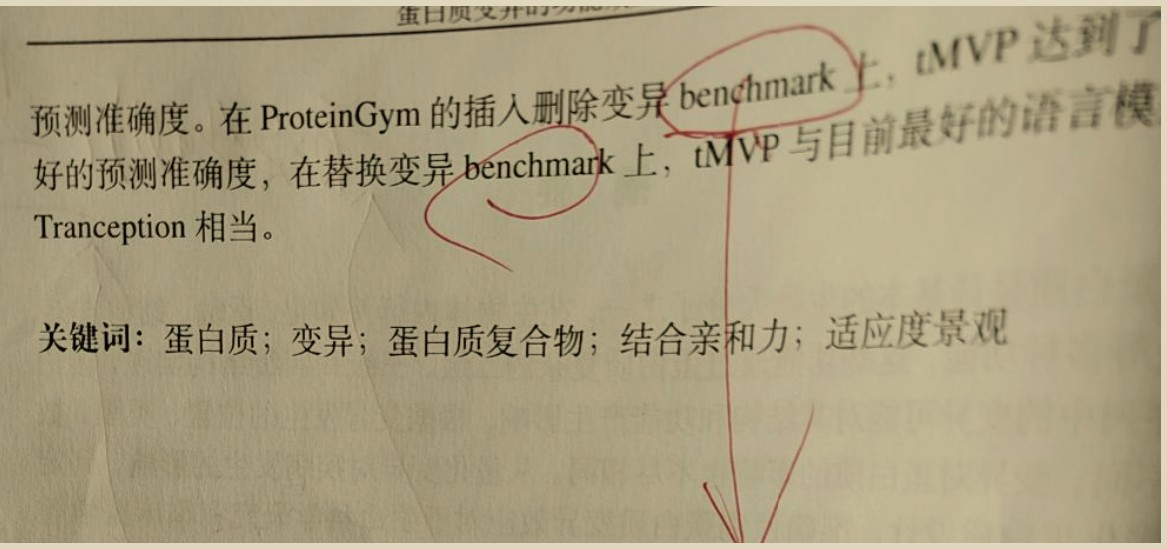
\includegraphics[scale=0.65]{doc/figures/chk05.jpg}
\caption{关键词分隔符}
\label{fig:keywords-sep}
\end{figure}
\end{itemize}





\section{英文缩写}
\begin{itemize}
\item \emph{首次出现英文缩写时,应采用“中文名(英文全称,缩写)”的格式;另,拉丁文要用斜体。比如大肠杆菌,应该写作“\textit{E. coli}”,中间有空格。}
\begin{figure}[!htpb]
\centering
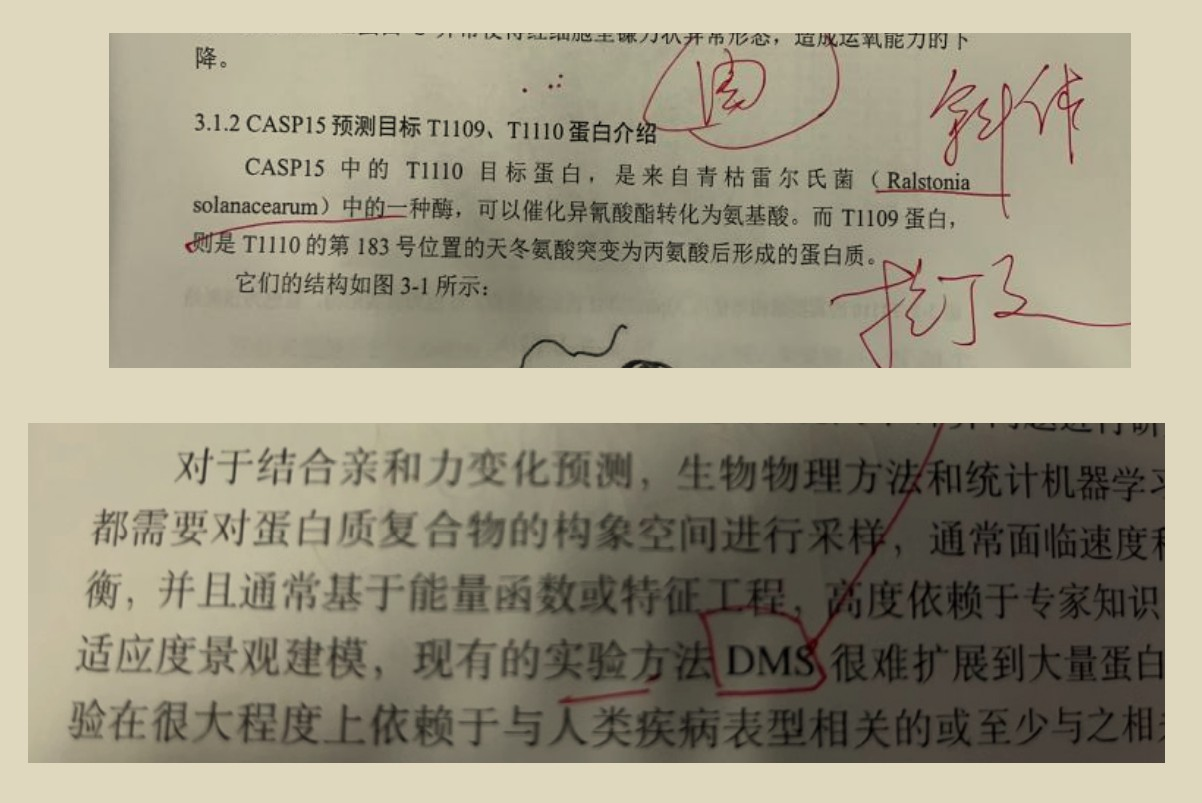
\includegraphics[scale=0.65]{doc/figures/chk03.jpg}
\caption{英文缩写格式错误}
\label{fig:abbrv-error}
\end{figure}
\end{itemize}

特殊名词或新名词应在适当位置加以说明或注解。双名法的生物学名部分均为拉丁文,并为斜体字。采用英语缩写词时,除本行业广泛应用的通用缩写词外,文中第一次出现的缩写词应该用括号注明英文原词。新的外来名词应用括号注
明英语全称和缩写语。



\section{中英文混杂}
\begin{itemize}
\item \emph{例如下图中的 benchmark,需要翻译成中文,不可中英混杂。另,常用的 Transformer 等都有规范译法。}
\begin{figure}[!htpb]
\centering
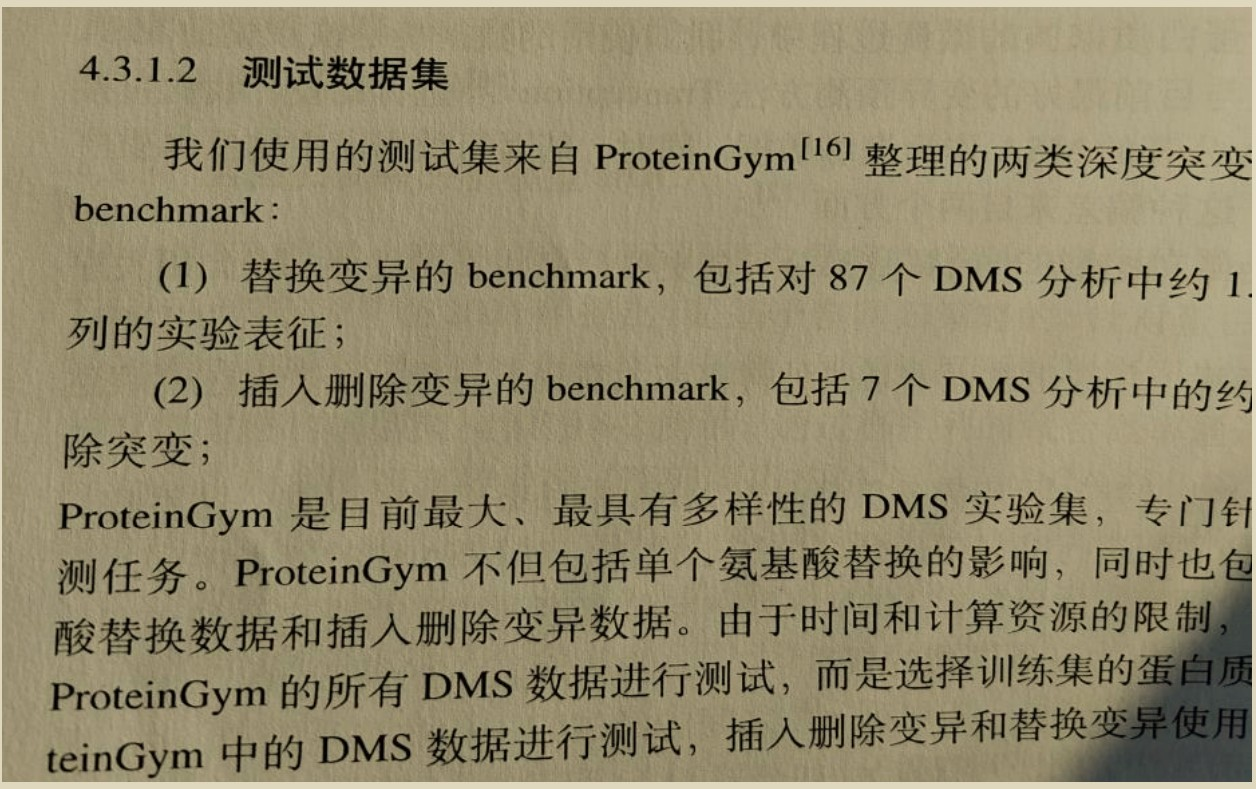
\includegraphics[scale=0.65]{doc/figures/chk04.jpg}
\caption{中英混杂错误}
\label{fig:mix-zh-cn-en-error}
\end{figure}
\end{itemize}




\section{避免含混}
不要出现易混淆词汇以及表示不明确句子。例如“序列”,讲清楚是“蛋白质序列”,不要以为读者靠上下文自然能够补足,要明确。再如“3.2.1 XYBind”中直接说 XYBind,读者会很糊涂;应该在前面加上“蛋白质-肽段相互作用预测算法 XYBind 的整体流程

\begin{figure}[!htpb]
\centering
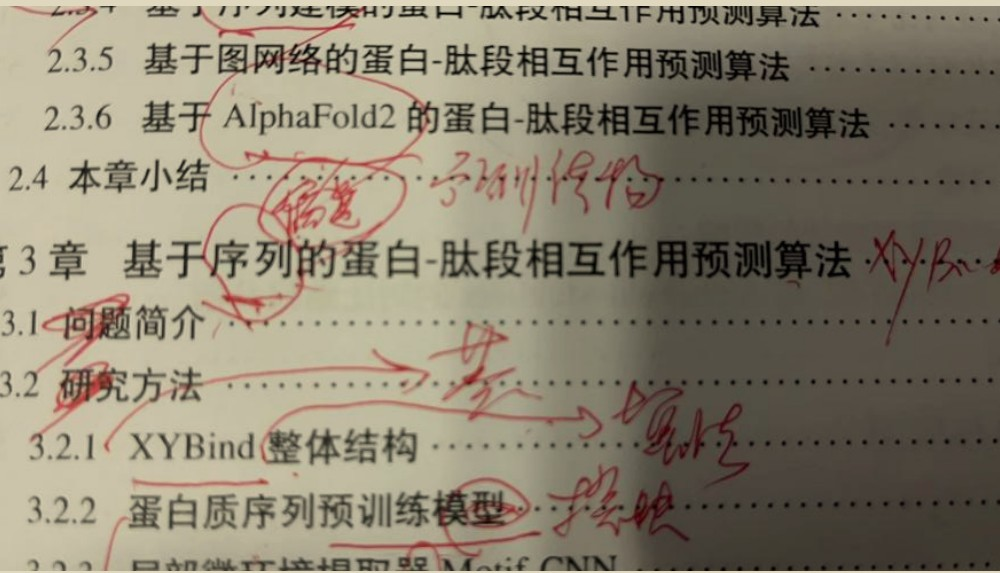
\includegraphics[scale=0.65]{doc/figures/chk06.jpg}
\caption{避免含混}
\label{fig:unclear-meanning}
\end{figure}


\section{公式排版}
\subsection{公式的转行}
关千数学式转行,1993年以前的国家标准没有做过明确的规定,大多数科技书刊在公式转行时遵循的是约定俗成的规则,即在 $=,+,-,/,\times,\cdot$ 等记号前转,并把这类记号放在下行行首。 

新标准对转行规则做出了明确的规定:“当一个表示式或方程式需要断开、用2行或多行来表示时,最好在紧靠其中记号$=,+,-,/,\times,\cdot,\pm$后断开,而在下一行开头不应重复这一记号。

读者看到上一行末尾的减号,就知道此式没有排完,下一行是由上一行转行来的,无论公式后面加不加点号,都不会产生误解。 这里的 “—”号,既是运算符号,又是连式符号,跟英文单词转行时需加的连字符所起的作用相同。至千转行的式子怎么排法,是居中排,还是与第1行的式子齐头,或是比第1行式子缩进几格;如果转行多次,转行的式子是否要左齐头排,或均居中排:新标准未作规定。 这些需要编辑根据版面设计要求和实际情况做出合理安排。




\subsection{公式的结尾}
数学式是用数字、字母和符号组合起来表达特定科学内容的,与文 字叙述具有同样的功能,是文章的有机组成部分。无论公式是串文排还 是居中排,在公式与公式之间,文字与公式之间,都要按实际需要确定 是否添加点号。公式尾部一定要加标点符号(英文)。如果公式所在的句子未结束,则使用逗号结尾,下一句不缩进;否则,以英文句号结尾,下一句要缩进。

下面的居中排公式后不应加点号:
\begin{example}
"……在比较一般的稳态黎曼时空
\begin{equation}
\mathrm{d} s^2 = g_{00} \mathrm{d} t^2  +  g_{11} \mathrm{d} x^2  +  g_{22} \mathrm{d} y^2  +  g_{33} \mathrm{d} z^2   +  2g_{03} \mathrm{d} t \mathrm{d} z  
\end{equation}
中,相对于视界……"
\end{example}

而下面的居中排公式后就需要加点号:
\begin{example}
"……式(XX)可写成
\begin{equation}
\hat{\rho} = \frac{1}{Z} \exp(-\beta ( \hat{H} - \Omega_{H} \hat{M})) \mbox{,}
\end{equation}
式中$\hat{H}$为……"
\end{example}


\subsection{公式 vs 程序}
公式就是公式,不能使用 Python 代码代替!

\begin{figure}[!htpb]
\centering
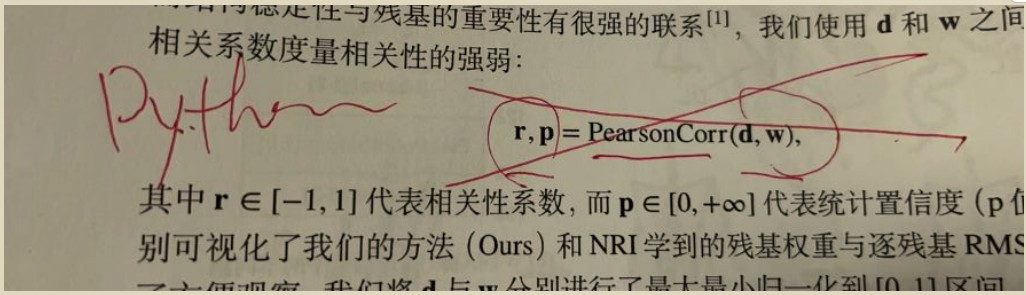
\includegraphics[scale=0.65]{doc/figures/chk08.jpg}
\caption{公式 vs 程序}
\label{fig:eqvscode}
\end{figure}


\section{表格}
表格的表头要用中文,不能用英文(如“Similarity”);数字一般情况下精确到小数点后 3 位,采用右对齐方式,以利于比较。

\section{图表的标题}
图表的标题要避免含混不清,不能指望读者从上下文猜测、补全出标题的含义,而应该是“含义自明的”,要突出与文章的关联;另,标题结尾不能出现标点符号。例如:图 2-3 的标题直接用“Social-LSTM”,比较突兀;应该前面加上短语以明示,比如改为“个体相互作用检查算法 Social-LSTM 中的社会力池化操作”,或者改成“基于……(社会力)模型……(任务)预测方法”。

各章标题中尽量不采用英文缩写词,对必须采用者,应使用本行业的通用缩写词,标题中尽量不使用标点符号。图应具有“自明性”,即只看图、图题和图注,不阅读正文,就可理解图意。每一图应有简短确切的图题,连同图序置于图下居中。

